\documentclass[compress]{beamer}
\usepackage{ifthen,verbatim}

\title{Muon HIP Alignment: mid-S156 update}
\author{Jim Pivarski, Alexei Safonov, K\'aroly Banicz$^*$}
\institute{Texas A\&M University, $^*$FermiLab}
\date{21 May, 2008}

\newcommand{\isnote}{}
\xdefinecolor{lightyellow}{rgb}{1.,1.,0.25}
\xdefinecolor{darkblue}{rgb}{0.1,0.1,0.7}

%% Uncomment this to get annotations
%% \def\notes{\addtocounter{page}{-1}
%%            \renewcommand{\isnote}{*}
%% 	   \beamertemplateshadingbackground{lightyellow}{white}
%%            \begin{frame}
%%            \frametitle{Notes for the previous page (page \insertpagenumber)}
%%            \itemize}
%% \def\endnotes{\enditemize
%% 	      \end{frame}
%%               \beamertemplateshadingbackground{white}{white}
%%               \renewcommand{\isnote}{}}

%% Uncomment this to not get annotations
\def\notes{\comment}
\def\endnotes{\endcomment}

\setbeamertemplate{navigation symbols}{}
\setbeamertemplate{headline}{\mbox{ } \hfill
\begin{minipage}{5.5 cm}
\vspace{-0.75 cm} \small
\end{minipage} \hfill
\begin{minipage}{4.5 cm}
\vspace{-0.75 cm} \small
\begin{flushright}
\ifthenelse{\equal{\insertpagenumber}{1}}{}{Jim Pivarski \hspace{0.2 cm} \insertpagenumber\isnote/\pageref{numpages}}
\end{flushright}
\end{minipage}\mbox{\hspace{0.2 cm}}\includegraphics[height=1 cm]{../cmslogo} \hspace{0.1 cm} \includegraphics[height=1 cm]{../tamulogo} \hspace{0.01 cm} \vspace{-1.05 cm}}

\begin{document}
\frame{\titlepage}

%% \begin{notes}
%% \item This is the annotated version of my talk.
%% \item If you want the version that I am presenting, download the one
%% labeled ``slides'' on Indico (or just ignore these yellow pages).
%% \item The annotated version is provided for extra detail and a written
%% record of comments that I intend to make orally.
%% \item Yellow notes refer to the content on the {\it previous} page.
%% \item All other slides are identical for the two versions.
%% \end{notes}

\begin{frame}
\frametitle{At a glance}
\begin{itemize}\setlength{\itemsep}{0.75 cm}
\item Full baseline-HIP procedure runs in S156
\item Results depend greatly on tracker misalignment (as expected)
\item We can identify good and bad alignments with data
\item Karoly solved his event-filtering problem and he is skimming
the MuonBeamHalo sample for CSC overlaps studies
\end{itemize}
%% \hspace{-0.83 cm} \textcolor{darkblue}{\Large Outline2}
\end{frame}

\begin{frame}
\frametitle{Parameters of alignment test}

\begin{center}
\begin{minipage}{0.5\linewidth}
For reference:

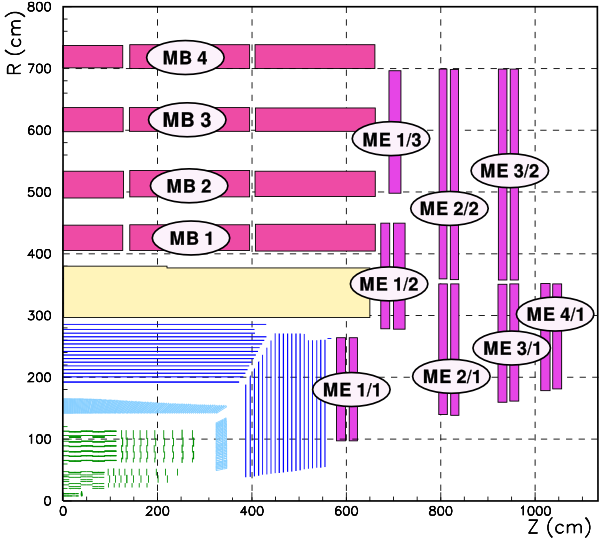
\includegraphics[width=\linewidth]{muon_system.png}
\end{minipage}
\end{center}

\begin{itemize}
\item Using $Z\to\mu\mu$, $W\to\mu\nu$, $\Upsilon\to\mu\mu$, $J/\psi\to\mu\mu$, MuonPT5, and MuonPT10
\item 17 jobs $\times$ 2 hours, merged with HIP's collector mode
\item Align to (a) ideal tracker and (b) results of S43 exercise
\end{itemize}
\end{frame}

\begin{frame}
\frametitle{Ideal tracker}

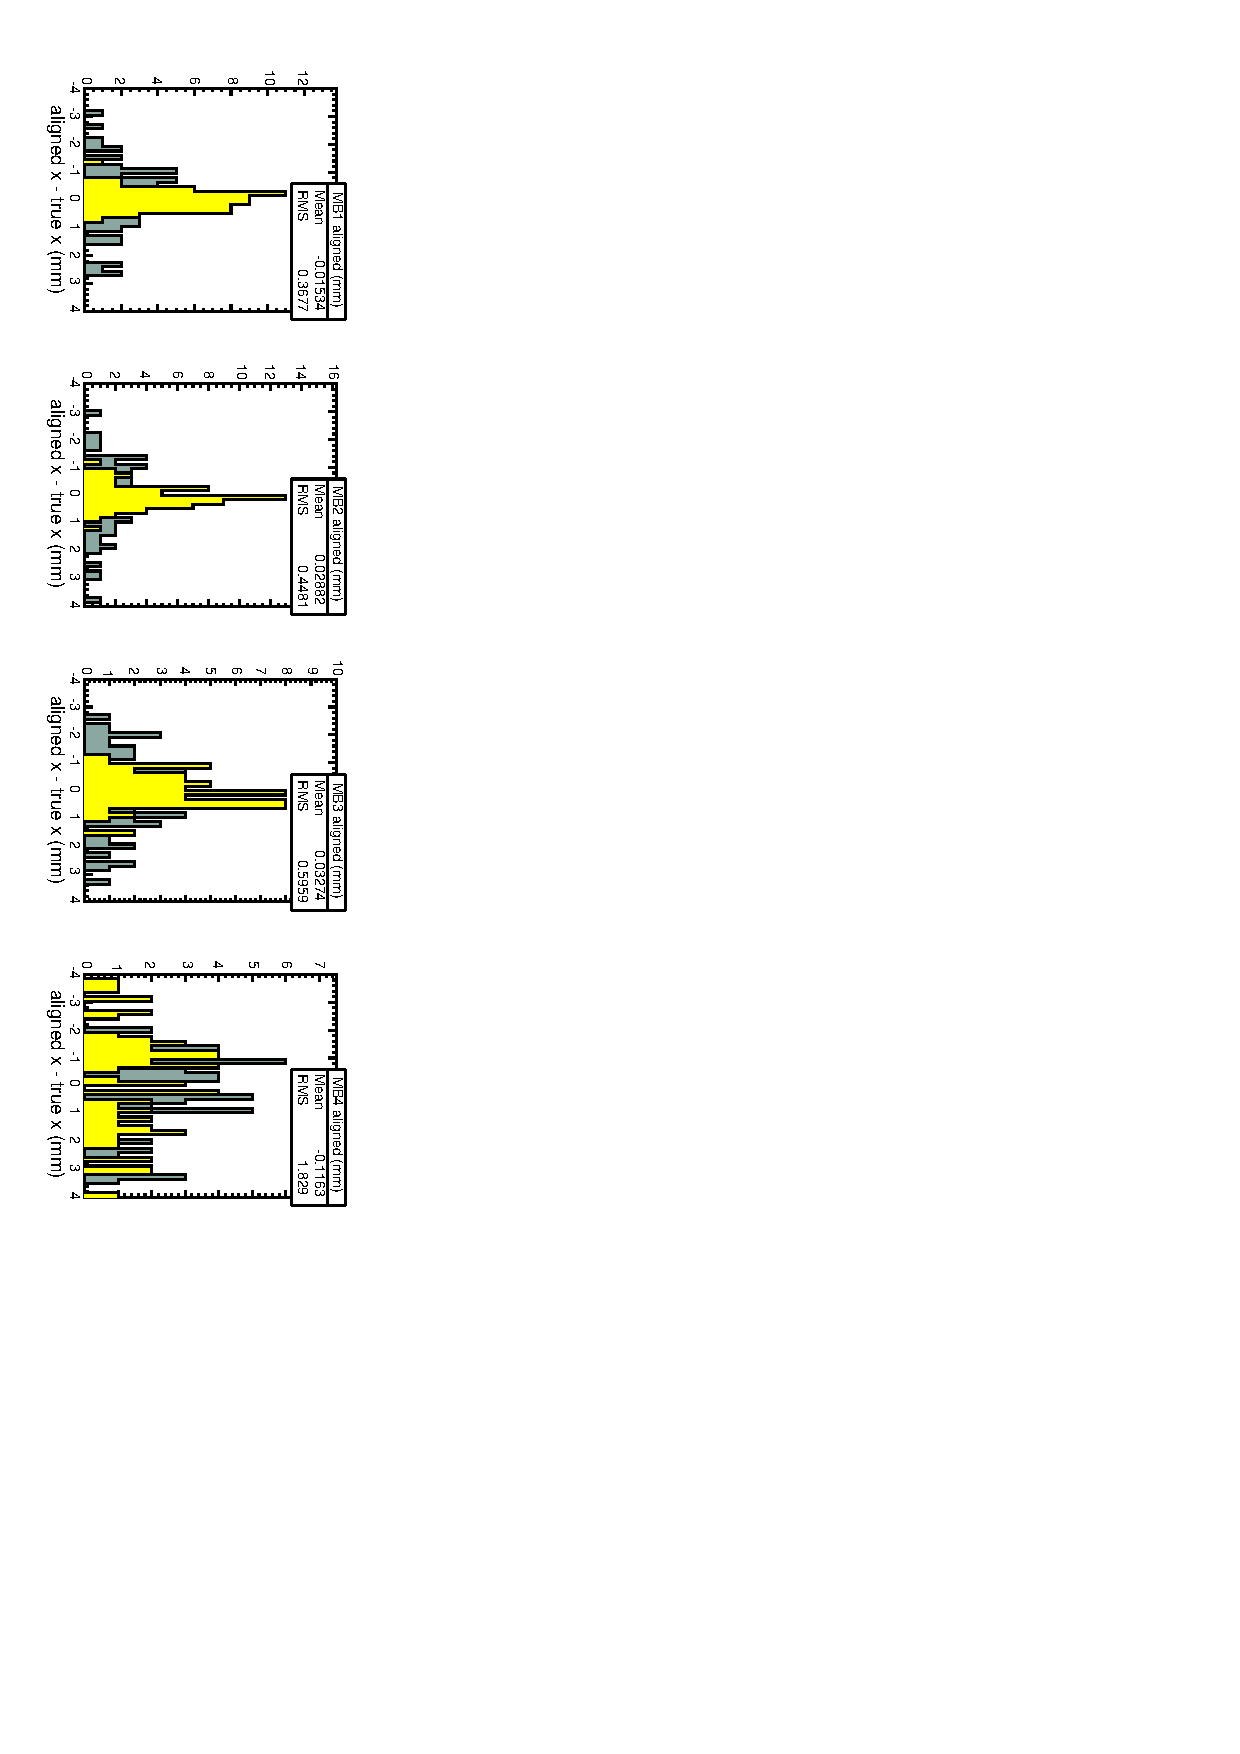
\includegraphics[height=\linewidth, angle=90]{idealtracker_barrelx.pdf}

\vfill
\hspace{-0.83 cm} \textcolor{darkblue}{\Large Misaligned tracker}

\vspace{0.5 cm}
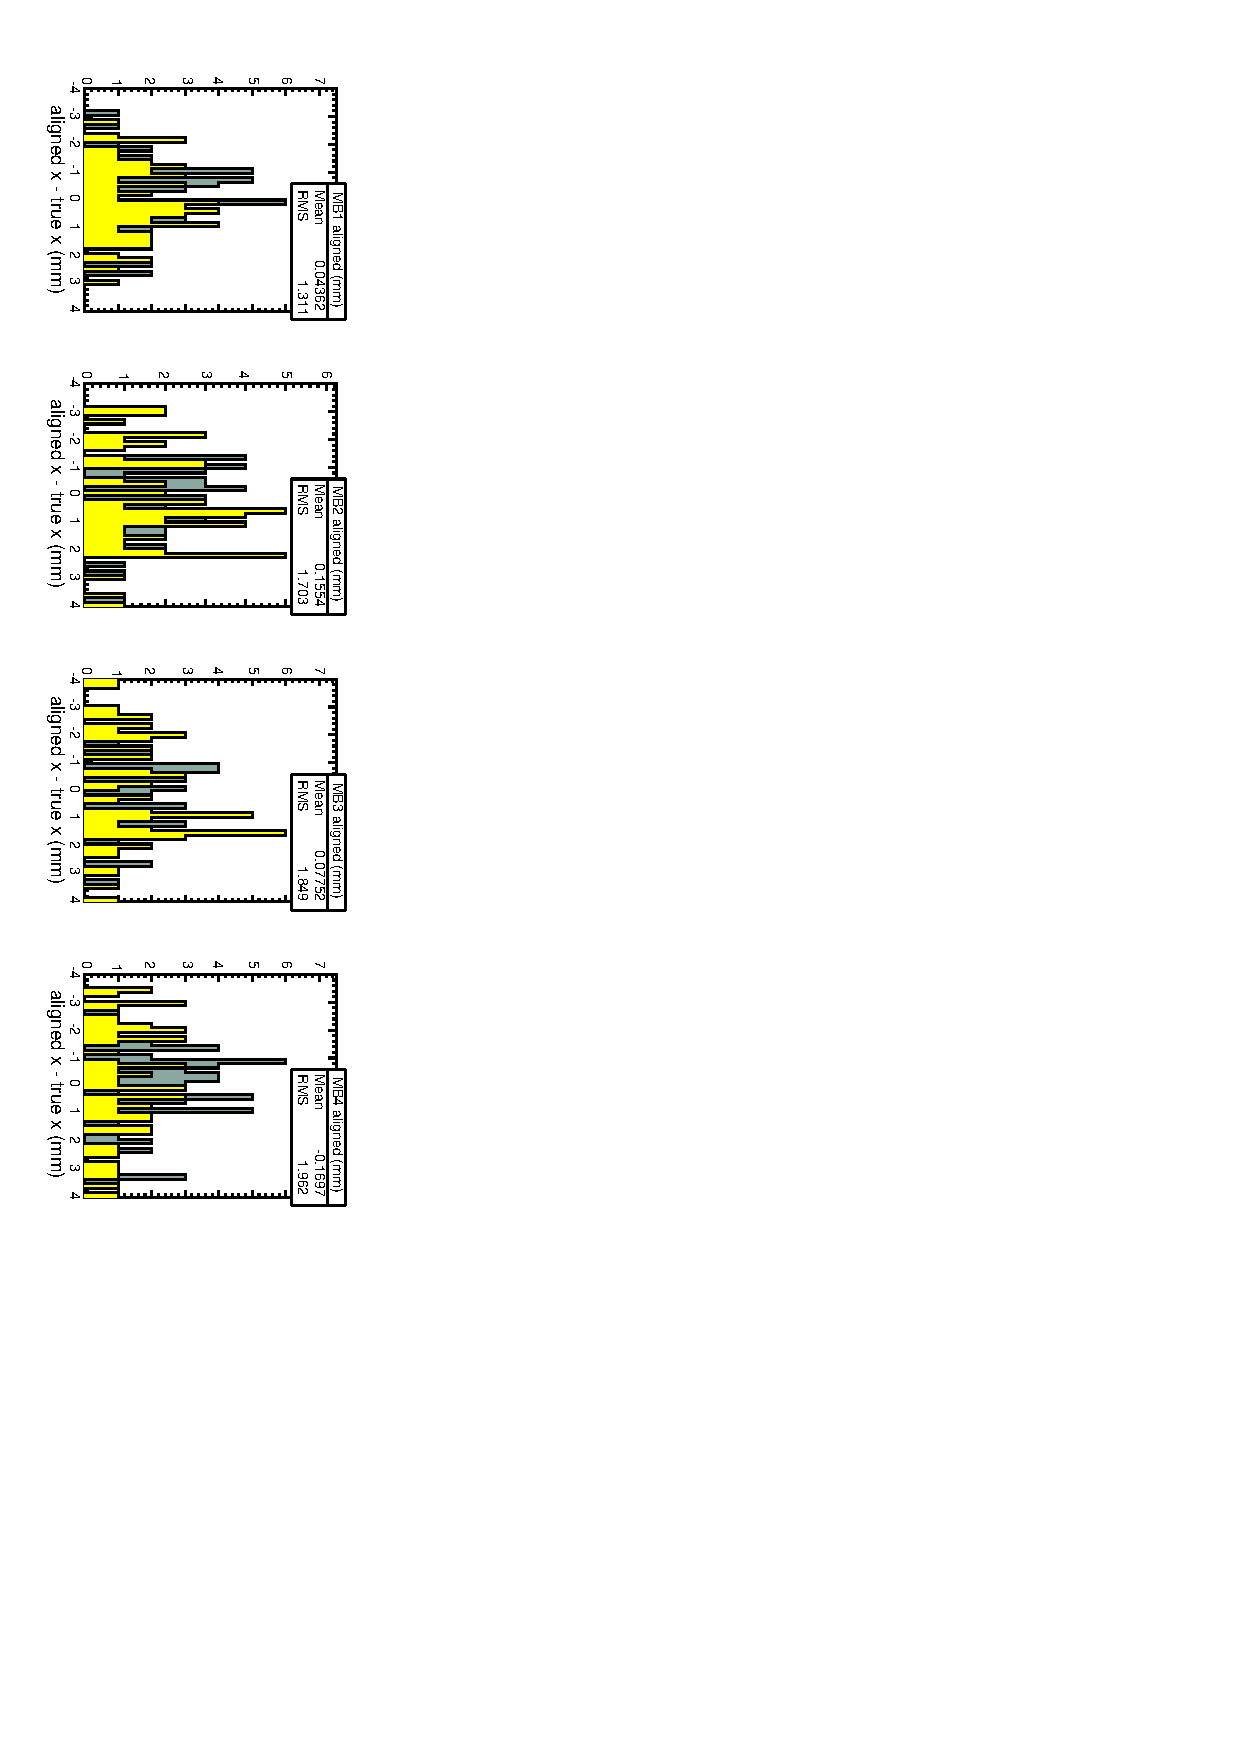
\includegraphics[height=\linewidth, angle=90]{real1ipb_barrelx.pdf}

\end{frame}

\begin{frame}
\frametitle{Ideal tracker}
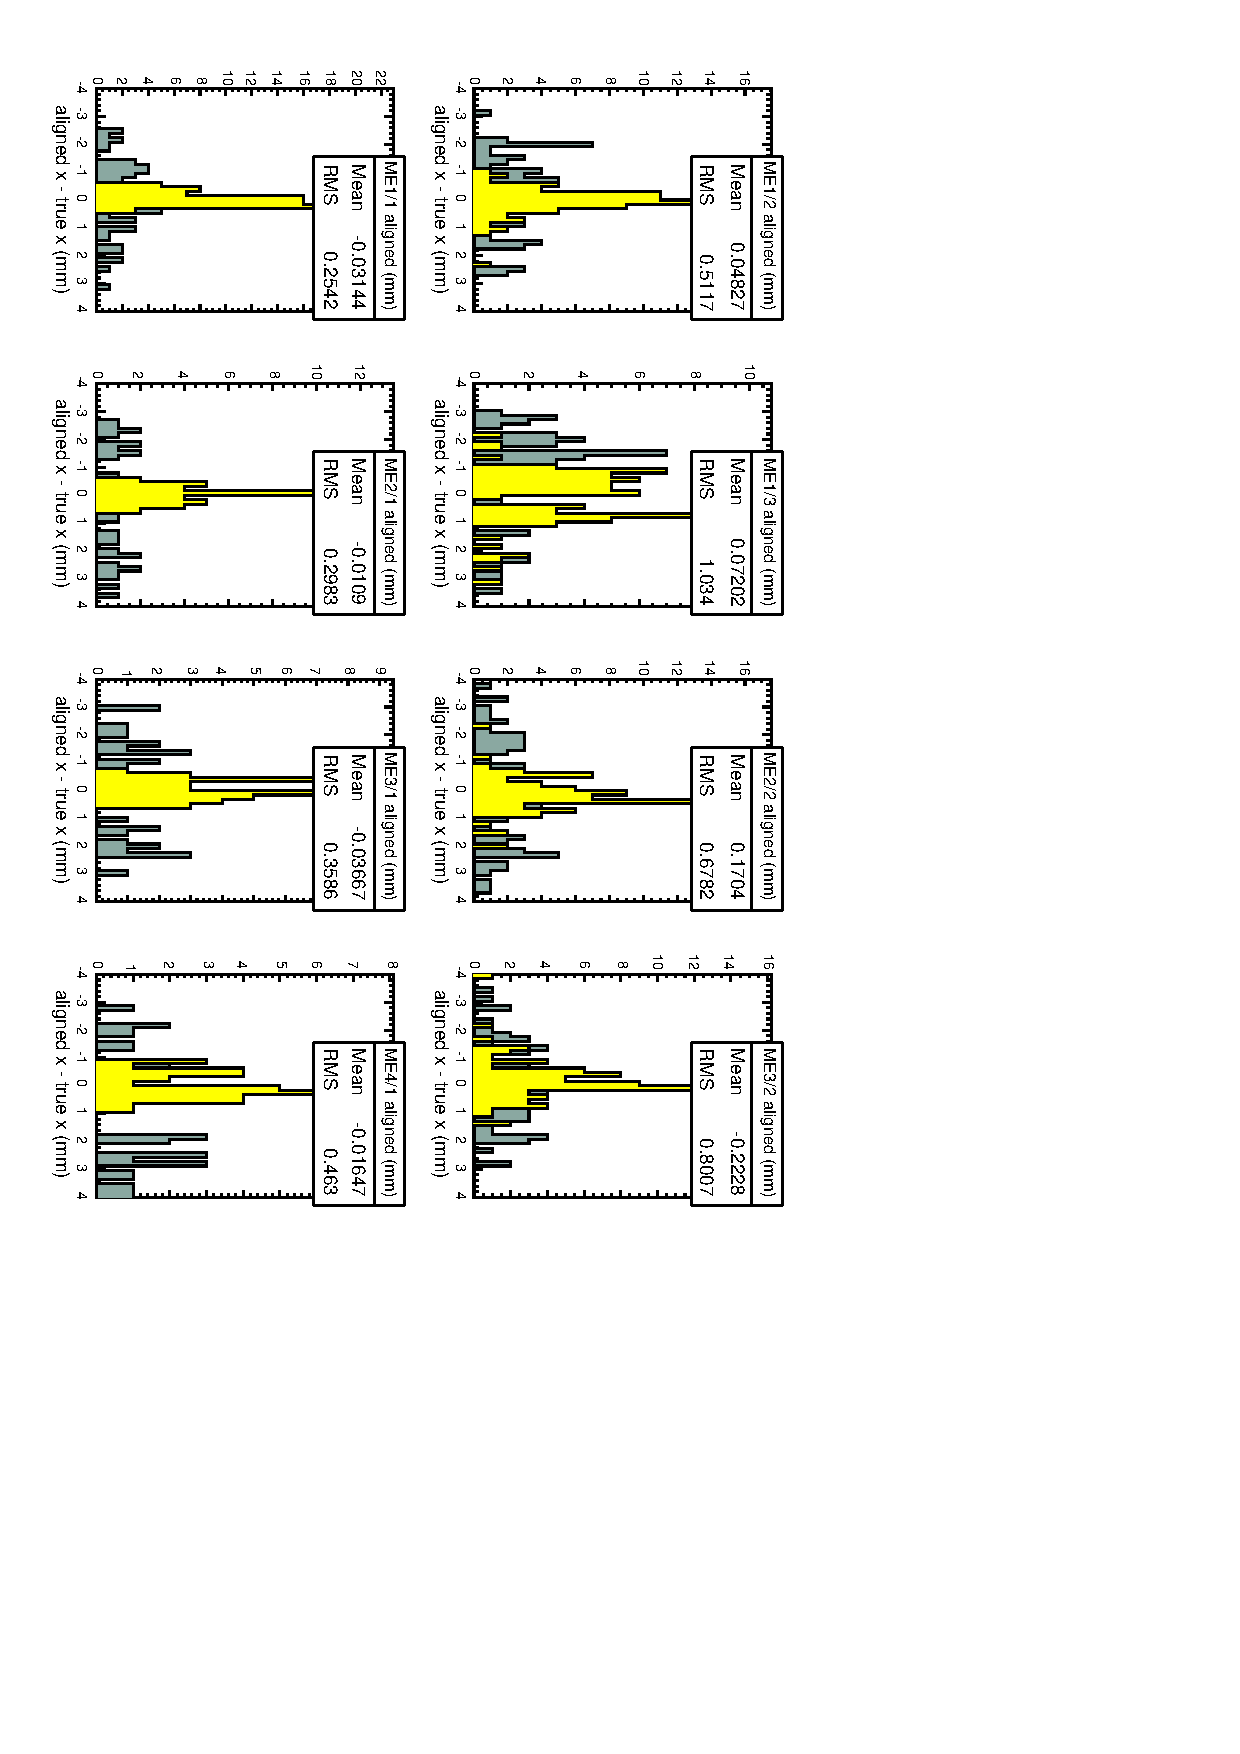
\includegraphics[height=\linewidth, angle=90]{idealtracker_endcapx.pdf}
\end{frame}

\begin{frame}
\frametitle{Misaligned tracker}
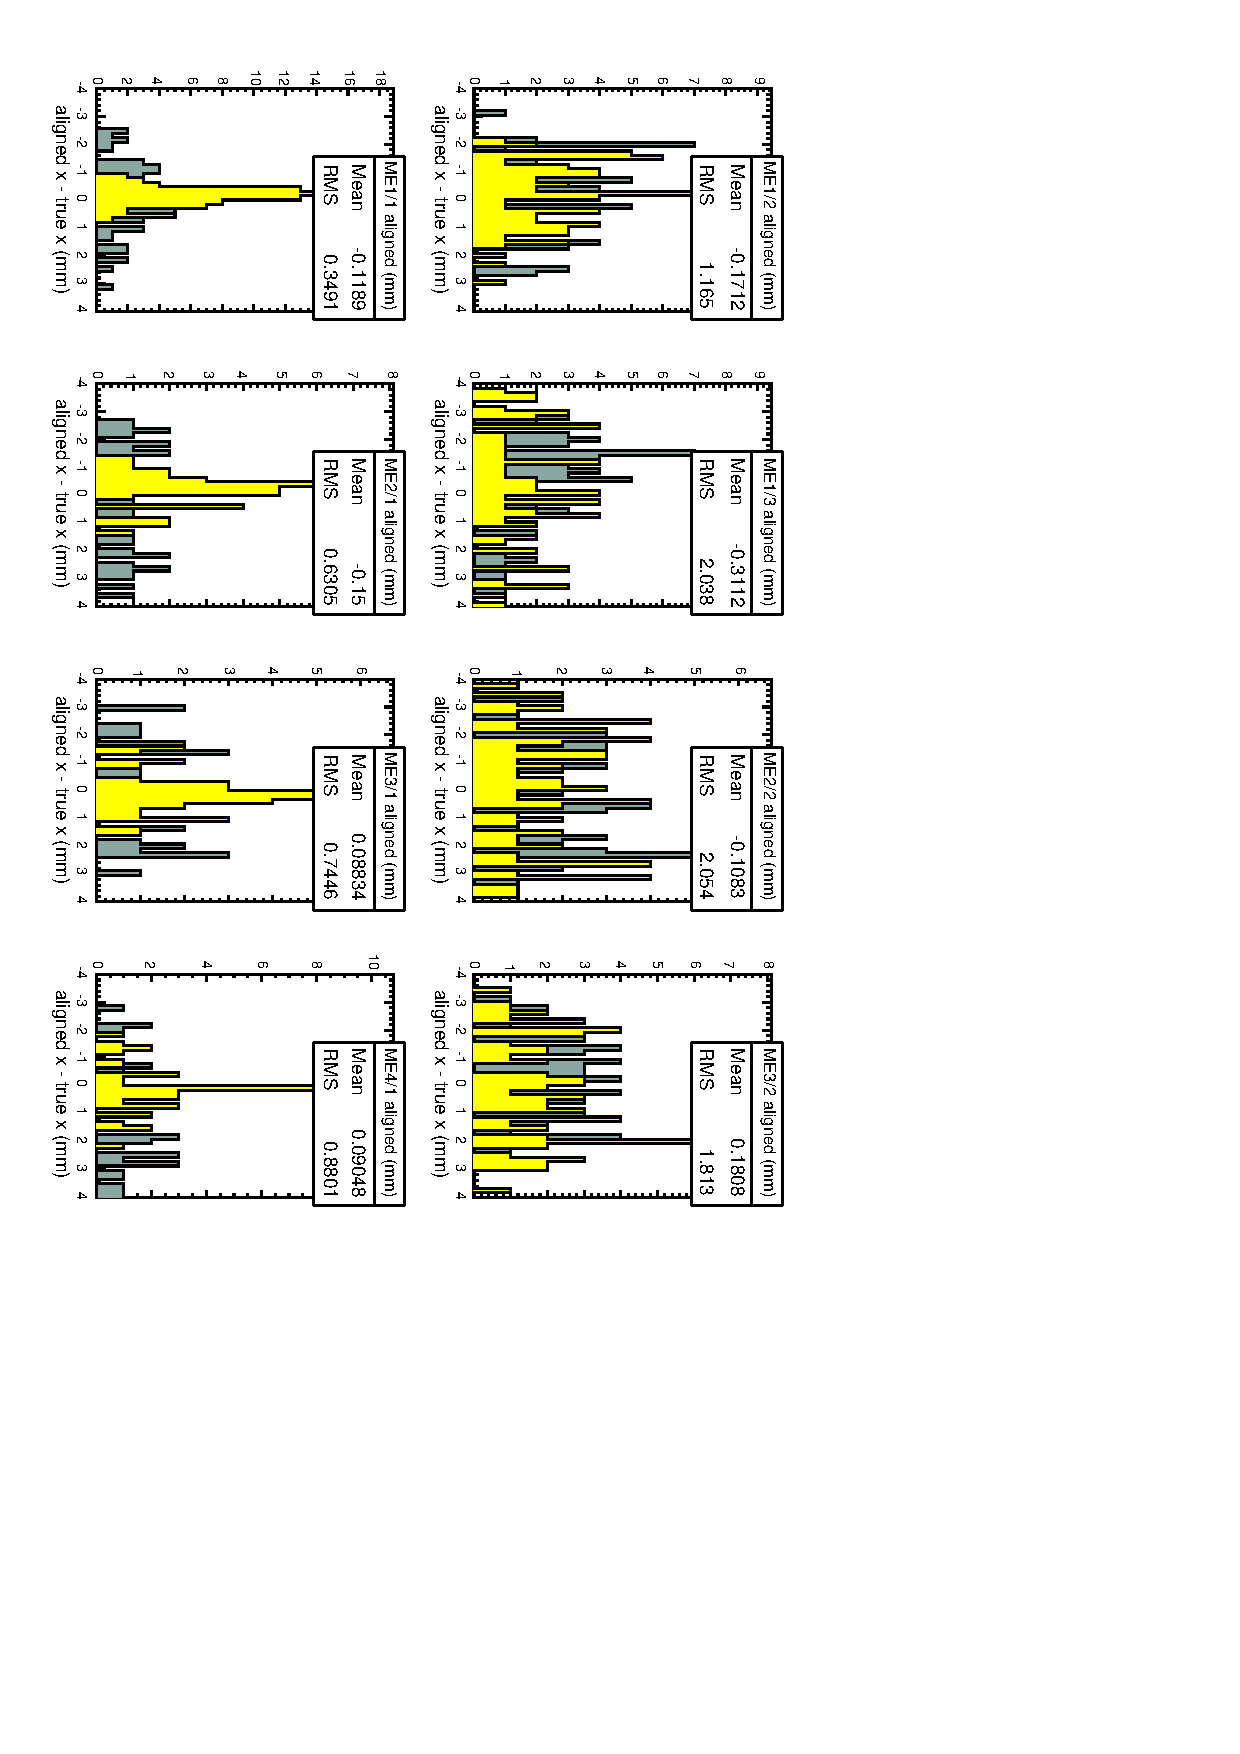
\includegraphics[height=\linewidth, angle=90]{real1ipb_endcapx.pdf}
\end{frame}

\begin{frame}
\frametitle{Selections from data}

\begin{itemize}
\item ``Figure of merit'' for a well-aligned chamber is $\mbox{stdev}/\sqrt{N}$
\item We can set a threshold for alignment based on this quantity:
chambers which do not meet it can be left untouched
\end{itemize}

\vspace{-0.25 cm}
\begin{center}
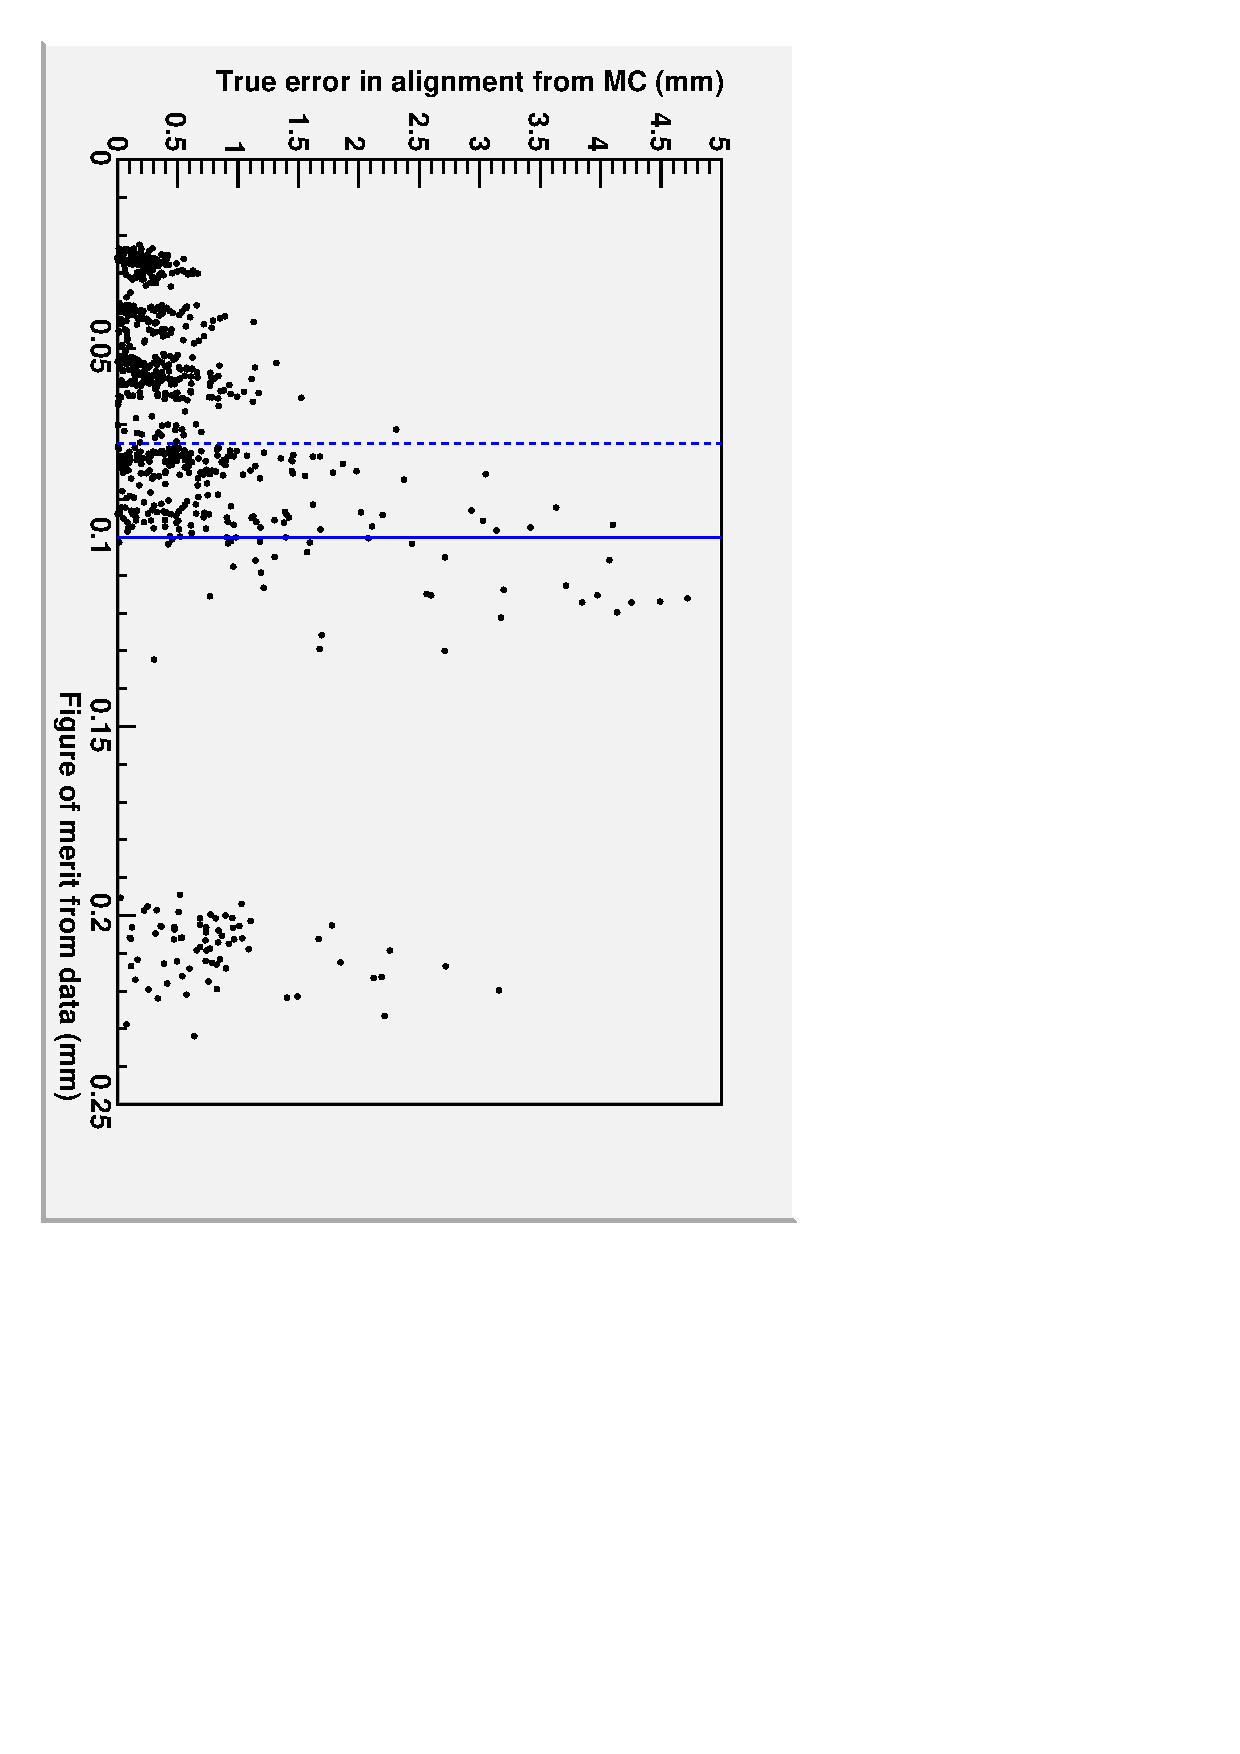
\includegraphics[height=0.8\linewidth, angle=90]{correlation_idealtracker.pdf}
\end{center}

\vspace{-0.25 cm}
\begin{itemize}
\item Blobs correspond to stations (ME1/3 on right)
\end{itemize}
\end{frame}

%% \section*{First section}
%% \begin{frame}
%% \begin{center}
%% \Huge \textcolor{blue}{First section}
%% \end{center}
%% \end{frame}

\begin{frame}
\frametitle{Next two days}

\begin{itemize}\setlength{\itemsep}{0.5 cm}
\item Try to determine whether muon alignment with a misaligned tracker would improve with statistics
\item Align muon system with tracker S156 geometry
\item \ldots and DT calibration (this is possible)
\item Take only the good chambers, produce an alignment, and validate it!
\end{itemize}

\label{numpages}
\end{frame}

\end{document}
